\documentclass{utue} %utue.cls required for Uni Tuebingen corporate design

\usepackage[style=numeric]{biblatex}
\addbibresource{bibliography.bib}
\usepackage{amsmath}

% Values for title generation
\title{Controlling Phasor Noise Artifacts}
\author{Jonathan Lang}
\date{\today}

% Subtitle is optional. It represents what kind of work you did.
\subtitle{Research Project}

\begin{document}

% You can place a teaser as follows. (Otherwise, just uncomment the following part)
%\teaser{
%    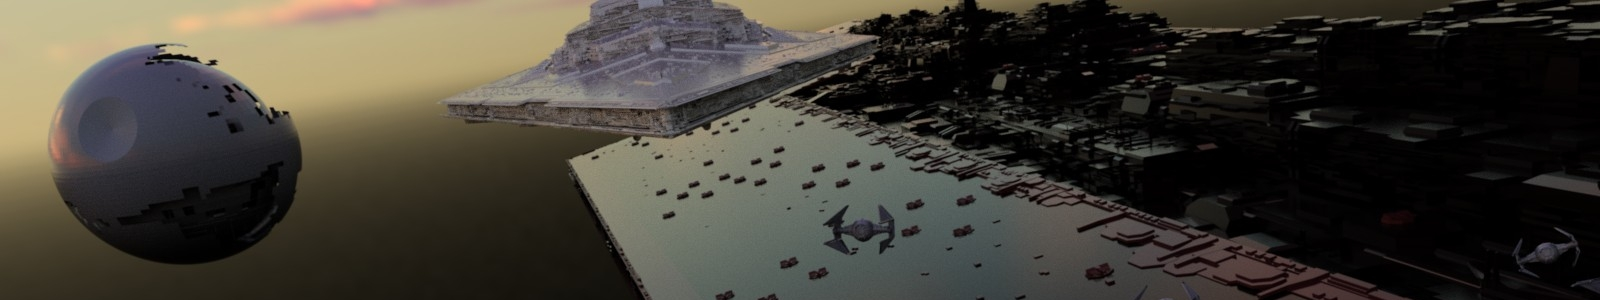
\includegraphics[width=\textwidth]{images/teaser.jpg}
%    \caption{\label{fig:teaser}You can place a teaser here.}
%}     

% Creates title of document and additional title page.
\maketitle 
 
\section*{Abstract}  
  
\section{Introduction}   
To keep up with the shorter development cycles of the current times more work has to be done in shorter time. The tools with which this is achieved are optimization of workflows as well as automation. While even the automation of repetitive tasks can be challenging, automating creative tasks like content creation is even more so. This is where noise algorithms provide assistance. They provide a way to generate non-repeating patterns over potentially infinite space at low memory and computational cost. Using these patterns two influence different aspect of the content, anything form additional detail on surfaces up to the layout of whole worlds can be generated automatically. The generated patterns are as varied as the algorithms itself. The different algorithms also provide different levels of influence over the produced pattern. Additional parameters to tune the generated pattern are of course desirable, as a richer set of patterns will be applicable for more situations, therefore offering further automation opportunities.


\section{Related Work}
Particularly interesting are anisotropic noise algorithms. As stated in \cite{survey}, these are noise algorithms produce patterns, whose appearance is not invariant to rotation. Besides providing definitions of most noise related terms \citeauthor{survey} also provide an overview of current Noise algorithms. The noise algorithm proposed by \citeauthor{anisotropicNoise} in \cite{anisotropicNoise} is actually not developed to produce interesting patterns with a discernible direction, but to enable the production of filtered noise to prevent aliasing when the noise texture is viewed at an angle. Today the term \textit{anisotropic noise} is more commonly used to refer to noise algorithms, which set out to produce and oriented pattern instead of ones with integrated filtering. One of these algorithms is the one proposed by \citeauthor{randomPhaseNoise} in \cite{randomPhaseNoise}. \citeauthor{randomPhaseNoise} produce noise by placing cosine with random phase, direction and frequency at grid points. By adjusting the way these random values are generated, the power spectrum of the noise can be precisely controlled. The ability to precisely control the power spectrum is a property shared with Gabor Noise as introduced by \citeauthor{gaborNoise} in \cite{gaborNoise}. Gabor Noise is a sparse convolution noise using a poission point process to generate Dirac impulses that are convoluted with the Gabor kernel to produce the final noise. Since this process inherits the power spectrum of the Gabor kernel, which can be adjusted quite precisely, this affords good control over the power spectrum of the noise, especially when differing instances of the Kernel are used. Despite how powerful Gabor noise is, it is still not perfect. One Problem is exhibits is the areas of low contrast, that have never been explicitly specified. This is a conclusion \citeauthor{spectrumOfVariance} also come to. In \cite{spectrumOfVariance} they develop a tool to quantify this local loss of contrast, which they call the spectrum of variance. Based on this, they develop a technique to remove low contrast areas from any noise instance. This generality however is a draw back as much as an advantage, since it can not use any information about the noise generation to achieve lower computation times. This is exactly what \citeauthor{phasorNoise} do in \cite{phasorNoise}. We will later have a more in depth look at their work.\\
Another big advantage of Gabor noise is its ability to be generated on the surface directly. This does not involve any texture coordinates, so the resulting noise instance does not show any seams. This ability is sought for, as works like \cite{appearanceTextureSynthesis}, \cite{textureSynthesis} and \cite{stripes} show. The former present algorithms, that can synthesise textures directly on surfaces, while the latter addresses a more basic problem. This problem is to find a function on a surface, that varies along a given direction field with a given rate. This is another piece of work we will look at in the following section.

\section{Background}
To avoid confusion we will denote a scalar using a simple letter e.g. $a$. A vector will be denoted with an arrow above e.g. $\vec{u}$. A scalar or elementwise multiplication will be represented by $\cdot$ or the absence of an operator e.g. $a\cdot b=ab$ is the multiplication between $a$ and $b$. The operands of a scalar product will be surrounded by $\langle$ and $\rangle$ e.g. $\langle\vec{u},\vec{v}\rangle$ denotes the scalar product between the vectors $\vec{u}$ and $\vec{v}$.
\subsection{Gabor Noise}
Since Phasor Noise inherits most of the abilities of Gabor Noise we will have a look at Gabor Noise before discussing it. As already mentioned Gabor Noise is produced by convolving Dirac impulses placed by a Poisson point process with the Gabor kernel as shown in figure \ref{fig:gaborNoise}. The Gabor kernel $g$ is defined as
$$
g(\vec{x}) = e^{\frac{||\vec{x}||}{\sigma^2}}\cdot \cos{(f\langle\vec{u},\vec{x}\rangle)}
$$
where $f$ and $\vec{u}$ are frequency and direction of the kernel and $\sigma$ represents its width like it does for a Gaussian function. Since the other operand of the convolution is a sum of offset Dirac impulses, the convolution deteriorates to a sum of offset versions of the kernel. An instance of Gabor Noise $G$ can therefore be represented as
$$
G(\vec{x}) = \sum_ig(\vec{x}-\vec{p}_i)
$$
where $\vec{p}_i$ are the positions of the Dirac Impulses. \citeauthor{gaborNoise} also prescribe a random weight to each instance of the kernel. However since this is not relevant for the following discussion, we omit it here for convenience. Figure \ref{fig:gaborNoise} shows an instance of Gabor Noise. The depicted instance is a bilobe instance. This name stems from the appearance of its power spectrum, which is two Gaussian lobes positioned at the frequency and direction of the used kernel. Using different kernels at different positions leads to a more varied appearance. Since the power spectra add up (and are rescaled) this permits to specify a custom power spectrum. Beside this amount of control Gabor noise can of course be extended from two to three dimensional. However \citeauthor{gaborNoise} also present a way to generate Gabor Noise directly on the surface of objects, which allows for seamless texturing.

\begin{figure}[h]
  \centering
  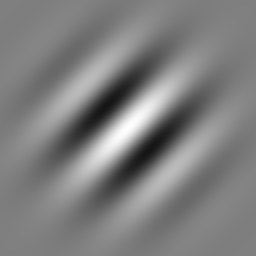
\includegraphics[width=0.45\linewidth]{images/gaborKernel}
  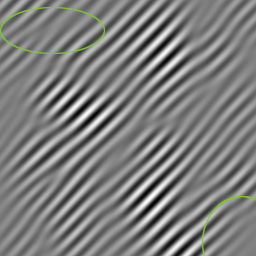
\includegraphics[width=0.45\linewidth]{images/gaborNoise}
  \caption{An instance of the Gabor Kernel (left) and an instance of Gabor Noise (right). Note the low contrast areas (marked).}\label{fig:gaborNoise}

\end{figure}

\subsection{Spectrum of Variance}
Gabor Noise however exhibits areas of low contrast, as figure \ref{fig:gaborNoise} shows. In \cite{spectrumOfVariance} \citeauthor{spectrumOfVariance} develop a tool to quantify these areas. They call this tool the spectrum of variance. As the name suggests for a given signal $s(\vec{x})$ the spectrum of variance $\mathcal{S}(s)$ is defined as
$$
\mathcal{S}(s) = \mathcal{F}((s-\overline{s})^2)
$$
where $\mathcal{F}$ denotes the Fourier transform and $\overline{s}$ represents the mean of the signal. Any nonzero values nearer than a distance $l$ to the origin correspond to low contrast areas bigger than $l$ in the original signal. As already mentioned, they also propose a process to remove these low contrast areas, namely by normalizing with the windowed standard deviation. However this normalization requires to compute the windowed standard deviation, which requires to evaluate the noise in the windows used. This leads to a big increase in computational cost, which is a significant drawback of this technique.

\subsection{Phasor Noise}\label{sec:phasorNoise}
We already mentioned, that the drawback of the normalisation technique proposed by \citeauthor{spectrumOfVariance} stems from the fact, that they can not use noise algorithm internal information. The logical conclusion is, that the only way to get a normalized noise texture without a big computation overhead is to design a variation of the algorithm, that produces normalized images. This is exactly what \citeauthor{phasorNoise} do in \cite{phasorNoise} for Gabor Noise. They realize, that for a signal of the form $s(x) = f(x)\cdot g(x)$, where $g$ is an oscillating function and $f$ is the envelope of $s$, discarding $f$ leads to a perfectly normalized signal. They then proceed to reformulate the bilobe case of Gabor Noise to have a form
$$
G(\vec{x}) = I(\vec{x})\sin{(f\langle\vec{x},\vec{u}\rangle + \varphi(\vec{x}))}
$$
where $f$ and $\vec{u}$ are again the frequency and direction of the main oscillation. $I$ is the envelope of the function and $\varphi(\vec{x})$ is the local phase offset of the oscillating part. The way they define $I$ and $\varphi$ this formulation is exactly equivalent to the corresponding Gabor Noise Instance. The main tool they use to do this is Phasor addition, hence the name Phasor Noise. Now, like in our example, we can discard the envelope $I$ to obtain a normalized version of Gabor Noise. \citeauthor{phasorNoise} call this a Phasor Sine wave. The actual Phasor Noise is the argument of the sine. Therefore Phasor Noise itself can not be used directly, but can only be used as input for a periodic function. Because it is defined using its corresponding Gabor Noise instance, it inherits the desirable properties of Gabor Noise, namely being band limited and a surface noise formulation. However, as depicted in figure \ref{fig:phasorNoise}, Phasor Noise exhibits several artifacts previously masked by the low contrast areas. There are two types of artifacts: singularities, where one stripe splits into two and what we will call rips, where the stripes are suddenly offset by some amount. Our goal will be to gain control over these artifacts to allow finer adjustments to the appearance of the noise.

\begin{figure}[h]
  \centering
  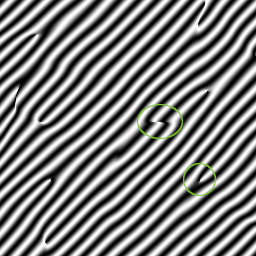
\includegraphics[width = 0.45\linewidth]{images/phasorSineWave}
  \caption{A Phasor Sine Wave. Note the artifacts previously masked by the low contrast areas.}\label{fig:phasorNoise}
\end{figure}

\subsection{Stripes Patterns on Surfaces}
In section \textcolor{red}{missing} we will see, that we need a function, defined on a mesh, that increases with a direction and speed determined by a vector field. We need this function to generate a stripe pattern by plugging it into a periodic function. As \citeauthor{stripes} already note, this is not alway trivial, even for a simple plane, as vector fields with non-zero curl are non integrable. In \cite{stripes} they provide a solution by deriving an equality constraint, that they than relax to a minimization. While necessary to receive a solution, it unfortunately allows new Singularities to emerge, which is obviously necessary, when considering a objects whose width varies along the stripe direction. As the width the stripes have to cover increases, either the number of stripes needs to increase, or the stripe frequency needs to drop. For our purposes one could replace their work with another way to generate a function that fulfills this purpose, but here we will use their work.

\section{The constant case}
We will first look at a simple case. This case corresponds to the bilobe case of Phasor Noise. This means a constant oscillation direction and frequency. However before we start out, we will define a third type of artifact besides singularities and rips: wobble. Comparing the areas of a Phasor Sine Wave with a regular Sine Wave, we find, that the lines are not perfectly straight. We will refer to this fact as wobble from no on. From section \ref{sec:phasorNoise} we recall that in this case Phasor Noise consists of two parts: A function increasing in a given direction and a phase offset. Figure \ref{fig:phasorNoisePhase} shows a Phasor Noise instance as well as its phase offset. Comparing the phase from figure \ref{fig:phasorNoisePhase} with figure \ref{fig:phasorNoise} we can easily find a correspondence between artifacts of the Phasor Sine Wave and feature of the phase. The existence of wobble is caused by the fact, that the phase is not constant even in areas, where there are no other artefacts present. \citeauthor{phasorNoise} already identify that rips are caused by sudden value changes in the phase offset, while singularities are located at points around which the phase offset rotates abruptly.\\

\begin{figure}[h]
  \centering
  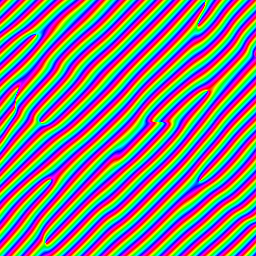
\includegraphics[width=0.45\linewidth]{images/phasorNoise}
  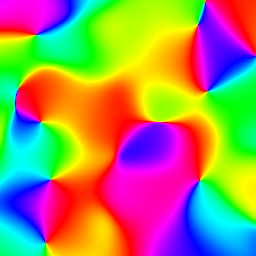
\includegraphics[width=0.45\linewidth]{images/phasorPhase}
  \caption{Phasor Noise (left) and its phase offset (right). Angle is mapped to hue.}\label{fig:phasorNoisePhase}
\end{figure}

This defines our goal. For a set of points $\vec{s}_i$, at which we want singularities to occur and a set of line segments $l_i$, along which we want rips to occur, we want to construct a varying phase offset $\varphi_c$ that suddenly changes when crossing any $l_i$ and abruptly rotates around all $\vec{s}_i$. Since this is a phase offset the numbers are considered module $2\pi$. Since wobble is the artifact most characteristic for Phasor Noise, we will assume that wobble is present in all applications, which will become relevant in section \textcolor{red}{missing}.

\subsection{Wobble}\label{sec:wobble}
The first artifact kind we will have a look at is wobble. As already mentioned, wobble is created by a non-constant phase. Since we are creating noise, we want this to be governed by randomness. Taking another look at figure \ref{fig:phasorNoisePhase}, we can not identify any obvious anisotropy. Therefore any noise algorithm whose appearance is not obviously anisotropic will be sufficient to create a similar appearance to Phasor Noise. An important to note is, that we do not use the fact, that the output domain is cyclic. There are two reasons for this is. The first is, that there is a multitude of noise algorithms with an equally large set of properties, that output to the real domain between $-1$ and $1$.\\
The other, more important one is that it is harder to ensure the absence of singularities when using a cyclic output domain. Take for example a simple algorithm that is based on an integer lattice and at each point of this lattice determines a random number and interpolates between them. Since we are using angles these random numbers will be between $0$ and $2\pi$. We are on a cyclic domain, so the interpolation will check if the points are nearer when using the normal difference or if they are nearer when computing the difference over the $0$/$2\pi$ boundary and choose the interpolation direction accordingly. We will now construct a possible case, where this algorithm will create singularity. This case is also shown in figure \ref{fig:simpleAlgirithmSingularity}. For this case choose a grid cell $C$ and its four corner points $p_1$, $p_2$, $p_3$ and $p_4$ in such a way, that $(p_1,p_2,p_3,p_4,p_1)$ moves along the edges around the cell. Now let the algorithm pick $0$, $\frac{\pi}{2}$,$\pi$ and $\frac{3\pi}{2}$ for $p_1$, $p_2$, $p_3$ and $p_4$ respectively. Since we interpolate on a cyclic domain, the points on the edge $(p_4,p_1)$ will be assigned value interpolated between $\frac{3\pi}{2}$ and $0$. We therefore created a path with a winding number of $1$ and therefore according to \textcolor{red}{some source} this path contains a singularity. Note, that this problem is not easily fixed, without removing the cyclic interpolation.\\
\begin{figure}[h]
  \centering
  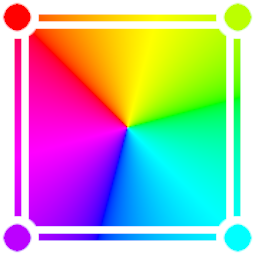
\includegraphics[width=0.45\linewidth]{images/simpleAlgo}
  \caption{A simple noise algorithm creating a singularity on a cyclic domain. The circles represent the points of the lattice while in between them the interpolation is shown. The rest shows possible values for the domain. Angle is again mapped to hue.}\label{fig:simpleAlgirithmSingularity}
\end{figure}
Therefore we will stick with algorithms outputting to the classic domain of $[-1,1]$. The actual phase offset is of course still in the cyclic domain on $[0,2\pi)$, so a value of minus one would wrap around to create the value $2\pi - 1$. When more or less wobble is needed these numbers can of course be rescaled to fit the specific needs. Figure \ref{fig:wobble} shows a Phasor Sine Wave with a phase offset applied. This phase offset is generated using a simple hierarchical algorithm, that uses cosine interpolation between lattice points. Note, that while there is an obvious difference in the phase offset used in figure \ref{fig:wobble} and the phase obtained from real Phasor Noise as shown in figure \ref{fig:phasorNoisePhase}, there is no noticeable difference in wobble when applied to a Phasor Sine Wave as shown in figure \ref{fig:phasorNoise}.
\begin{figure}[h]
  \centering
  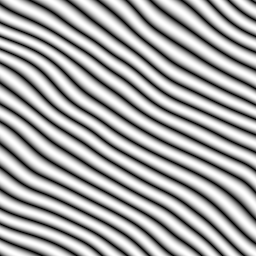
\includegraphics[width=0.45\linewidth]{images/wobble}
  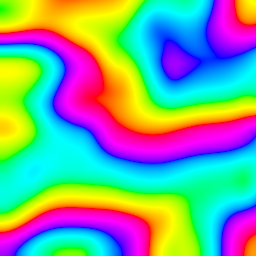
\includegraphics[width=0.45\linewidth]{images/wobblePhase}
  \caption{An artificially created Phasor Sine Wave (left) without any artifacts except for wobble and its phase offset (right).}\label{fig:wobble}
\end{figure}
When using the function $w(\vec{x})$ to compute the phase offset causing the wobble, we can represent our constructed phase offset as $\varphi_c(\vec{x}) = w(\vec{x})$.

\subsection{Singularities}
As we already found, singularities are located at points, where the phase offset rotates rapidly. To construct singularities, we therefore need to construct these points in the phase offset. To achieve this, we will (literally) add another component to the generated phase offset. Given the polar coordinates $(r, \theta)$ of a point $\vec{x}$ we can use the function
$$
atan(\vec{x}) = \begin{cases}
  0 & \text{if } r = 0\\
  \theta &\text{otherwise}
\end{cases}
$$
Figure \ref{fig:singularities} shows this function as well as its impact when used as a phase offset for a sine wave. It also shows $-atan(\vec{x})$ and its impact when used as phase offset. We can clearly see a difference in Phasor Sine Wave. Along the direction from the top left to the bottom right, $atan(\vec{x})$ leads to an additional line, while $-atan(\vec{x})$ removes a line. This clearly indicates a need to differentiate between the two. We will call the first one a right singularity, while we will call the second one a left singularity. Recalling from our goal, we want singularities at points $\vec{s}_i$. Since we now need to differentiate between the two types of singularities, we will continue to denote points of right singularities by $\vec{s}_i$, while we will denote points with left singularities by $\vec{t}_i$. Using this, we can expand our constructed phase by to 
$$
\varphi_c(\vec{x}) = w(\vec{x}) + \sum_i atan(\vec{x}-\vec{s_i}) - \sum_j atan(\vec{x}-\vec{t_j})
$$
\begin{figure}[h]
  \centering
  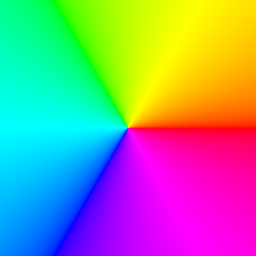
\includegraphics[width=0.23\linewidth]{images/rightSingularityPhase}
  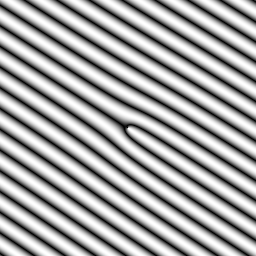
\includegraphics[width=0.23\linewidth]{images/rightSingularity}
  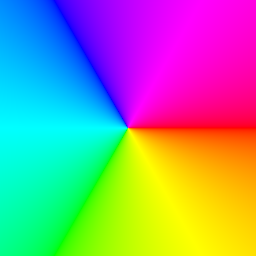
\includegraphics[width=0.23\linewidth]{images/leftSingularityPhase}
  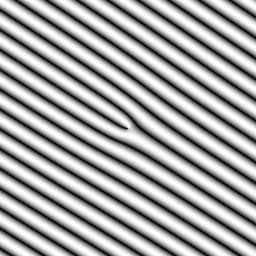
\includegraphics[width=0.23\linewidth]{images/leftSingularity}
  \caption{A simple way to add a single singularity to a sine wave. In order: Phase offset of right singularity, right singularity in Phasor Sine Wave, phase offset of left singularity, left singularity in Phasor Sine Wave. Both Phasor Sine Waves are without wobble. For the phase offsets angle is mapped to hue.}\label{fig:singularities}
\end{figure}

One important thing to note is the fact, that this means, that for each point we need to evaluate each of the singularity terms. For large images with a lot of singularities this will slow down the evaluation a lot.


\printbibliography


\end{document}

